%\documentclass[9pt,handout]{beamer}
\documentclass[11pt]{beamer}

%\usepackage[style=alphabetic]{biblatex}

%\usepackage{pgfpages}
%\setbeameroption{show notes on second screen=left}

% Copyright 2004 by Till Tantau <tantau@users.sourceforge.net>.
%
% In principle, this file can be redistributed and/or modified under
% the terms of the GNU Public License, version 2.
%
% However, this file is supposed to be a template to be modified
% for your own needs. For this reason, if you use this file as a
% template and not specifically distribute it as part of a another
% package/program, I grant the extra permission to freely copy and
% modify this file as you see fit and even to delete this copyright
% notice.
%
% Modified by Tobias G. Pfeiffer <tobias.pfeiffer@math.fu-berlin.de>
% to show usage of some features specific to the FU Berlin template.

% altered by someone at TU. fiddled with and fixed some things by 
% Nicolas Werner (some UTF-8 fix, biblatex-biber intro before toc,
% other stuff I can't remember)

% remove this line and the "ucs" option to the documentclass when your editor is not utf8-capable
\usepackage[utf8]{inputenc}
\usepackage[T1]{fontenc}   % to make utf-8 input possible
\usepackage[english]{babel}     % hyphenation etc., alternatively use 'german' as parameter
\usepackage{verbatim}           % comments and stuff
\usepackage[right]{eurosym}
\usepackage{booktabs}
\usepackage{tikz}
\newcommand{\todo}[1]{\raisebox{0pt}{\parbox{0pt}{\begin{large}\colorbox{red}{todo: #1}\end{large} \hspace*{0.05cm}}}}

\usepackage{blindtext}
\usepackage[fixlanguage]{babelbib}
\selectbiblanguage{english}


% ``English''  <>  "`Deutsch"'
\newcommand{\germanQuote}[1]{\glqq#1\grqq}
\newcommand{\englishQuote}[1]{``#1''}
% in Überschriften kann es sein,
% dass man danach $\;$ 
% setzen muss, damit
% die Abstände stimmen.....
% in Sections ist das aber illegal
% deswegen:
% \texorpdfstring{\germanQuote{Text} $\;$blah}{\germanQuote{Text} blah}

%\addbibresource{references.bib}
\bibliographystyle{alpha}
%\bibliography{references}

\include{tu-beamer-template}  % THIS is the line that includes the TU template!
% Quelle: http://tex.stackexchange.com/questions/56417/list-of-figures-beamer
\usepackage{ifthen}
\usepackage{xstring}

\makeatletter

%\defbeamertemplate*{caption label separator}{colon}{:}

\def\dotfill{%
  \leavevmode
  \cleaders \hb@xt@ .44em{\hss.\hss}\hfill
  \kern\z@}

\newcommand{\myVL}[2]{\tmpVL{#1}{#2}}

\newcommand{\tmpVL}[2]{Page #1, last accessed: #2}

\newcommand{\myhref}[2]{\tmphref{#1}{#2}}

\newcommand{\tmphref}[2]{\href{#1}{Source}, last accessed: #2}

\AtEndDocument{%
  % sorgt dafür, dass die Dateien 
  % *.lof -> list of figures
  % *.lot -> list of tables
  % geeleert werden oder ggf. neu erzeugt werden (erzwungen)
  \clearpage
  \beamer@tempcount=\c@page\advance\beamer@tempcount by -1%
  \if@filesw
  \newwrite\tf@lof
  \immediate\openout\tf@lof\jobname.lof\relax
  \newwrite\tf@lot
  \immediate\openout\tf@lot\jobname.lot\relax
  \fi
}

% beamer caption ändern....
\long\def\beamer@makecaption#1#2#3#4{%
  % [ von caption selbst]
  % #1 == Typ == Bild / Tabelle....
  % #2 == optionale Beschreibung
  % #3 == caption Beschreibung
  % bsp: \caption[optionale Beschreibung]{caption Beschreibung}

  % calls: \beamer@makecaption{#1}{\ignorespaces #3}{yes/no}{\ignorespaces #2}  

  % ----------------------------------------------

  % #1 == Typ == Tabelle / Bild.....
  % #2 == Captionbeschreibung
  % #3 == yes/no if you want complete Text under picture
  % #4 == optionale Beschreibung vom Bild
  \hypertarget{\insertframenumber}{}{}
  % \def\insertcaptionname{\csname#1name\endcsname}%
  % liefert Figure, weil babel auf englisch....
  \def\insertcaptionname{Fig.}%
  \def\insertcaptionnumber{\csname the#1\endcsname}%
  \edef\insertframenumber{\theframenumber}%
%  \ifthenelse{\equal{#3}{\empty}}{%  
    \def\insertlistcaption{#2}%
%  }{%
%    \def\insertlistcaption{#3}%
%  }
  	\def\insertsource{#4}%
    %
    \def\insertcaption{#2}%
    \ifthenelse{\equal{#1}{figure}}{%  
      \addtocontents{lof}{\relax\protect\listoffigureformat{\insertcaptionnumber}{\insertlistcaption}{\protect\hyperlink{\insertframenumber}{\insertframenumber}}{\insertsource}}{}{}%
      }{}
    \ifthenelse{\equal{#1}{table}}{%  
      \addtocontents{lot}{\protect\listoftableformat{\insertcaptionnumber}{\insertlistcaption}{\insertframenumber}}{}{}%
      }{}
  \ifthenelse{\equal{#3}{no}}
  { 
  	% Text beim Bild
    %\addtocontents{lof}{#4,jaaaaaaaaaaaaaaaaaaaaaaa}%
  	\nobreak\vskip\abovecaptionskip\nobreak
  	\sbox\@tempboxa{
  		%\usebeamertemplate**{caption}
  		%\raggedright
    	{%	
      		\usebeamercolor[fg]{caption name}%
      		\usebeamerfont*{caption name}%
      		\insertcaptionname~\insertcaptionnumber
    	}
    	\par
  	}%
  	\ifdim \wd\@tempboxa >\hsize
    	%\usebeamertemplate**{caption}\par
    	%\raggedright
    	{%
      		\usebeamercolor[fg]{caption name}%
      		\usebeamerfont*{caption name}%
      		\insertcaptionname~\insertcaptionnumber
    	}
    	\par
 	\else
  		\global \@minipagefalse
  		\hb@xt@\hsize{\hfil\box\@tempboxa\hfil}%
  	\fi
  	\nobreak\vskip\belowcaptionskip\nobreak%
  }{ 
	% Text beim Bild
    %\addtocontents{lof}{#4,jaaaaaaaaaaaaaaaaaaaaaaa}%
  	\nobreak\vskip\abovecaptionskip\nobreak
  	\sbox\@tempboxa{
  		%\usebeamertemplate**{caption}
  		%\raggedright
    	{%	
% % nw: figure numbering in slides
%      		\usebeamercolor[fg]{caption name}%
%      		\usebeamerfont*{caption name}%
%      		\insertcaptionname~\insertcaptionnumber
%      		\usebeamertemplate{caption label separator}%
    	}
    	\insertcaption\par
  	}%
  	\ifdim \wd\@tempboxa >\hsize
    	%\usebeamertemplate**{caption}\par
    	%\raggedright
    	{%
      		\usebeamercolor[fg]{caption name}%
      		\usebeamerfont*{caption name}%
      		\insertcaptionname~\insertcaptionnumber
      		\usebeamertemplate{caption label separator}%
    	}
    	\insertcaption\par
 	\else
  		\global \@minipagefalse
  		\hb@xt@\hsize{\hfil\box\@tempboxa\hfil}%
  	\fi
  	\nobreak\vskip\belowcaptionskip\nobreak%  }
  }
}

\def\listoffiguresectionformat#1#2{%
  % \listoffiguresectionformat{\insertsectionhead}{\insertframenumber}
  % #1 == Sectiontitel
  % #2 == Seite
  \setlength{\leftskip}{2ex}
  \setlength{\rightskip}{-0.6ex}
  \setlength{\parindent}{-3ex}
  %
  {\usebeamercolor[fg]{bibliography entry author} #1}%
  \dotfill%
  \hspace*{0.6ex}%
  \makebox[3ex][r]{#2}\par%
  %
  \setlength{\leftskip}{3ex}
  \setlength{\rightskip}{0ex}
  \setlength{\parindent}{-3ex}
}

\newcounter{tmpImageCounter}
\setcounter{tmpImageCounter}{0}

\def\listoffigureformat#1#2#3#4{%
	\ifnum\value{tmpImageCounter}=#1
		\typeout{Counter \thetmpImageCounter  ist gleich #1. Das Muss das erste Bild sein...}
		% \listoffigureformat{\insertcaptionnumber}{\insertlistcaption}{\insertframenumber}{\insertsource}
		% #1 == Bildnummer
		% #2 == Captionbeschreibung
		% #3 == Seite, wo das Bild ist
		% #4 == optionale Beschreibung vom Bild 
		% \caption[optionale Beschreibung]{Captionbeschreibung}
		\makebox[2ex][r]{#1}%
		\hspace{1ex}%
		{\usebeamercolor[fg]{bibliography entry author} #2}%
		\ifthenelse{\equal{#4}{\empty}}{}{ -- #4}%
		\dotfill%
		\makebox[3ex][r]{#3}\par%
		\refstepcounter{tmpImageCounter}
	% Bild wurde schonmal gesetzt....nee nicht nochmal...
  	\else
		\PackageWarning{listoffigureformat}{Bild wurde doppelt gesetzt -- wird ignoriert!}
		\typeout{Counter \thetmpImageCounter ist groesser oder kleiner #1.}
	\fi

}

% der eigentliche Befehl, der am Ende die Liste der Figures anzeigt
\def\listoffigures{%
  \setlength{\leftskip}{3ex}
  \setlength{\parindent}{-3ex}
  \@starttoc{lof}%
}

\def\listoftableformat#1#2#3{%
 % \listoftableformat{\insertcaptionnumber}{\insertlistcaption}{\insertframenumber}
 % #1 == Tabellennummer
 % #2 == Captionbeschreibung 
 % #3 == Seite, wo die Tabelle ist
 \makebox[2ex][r]{#1}\hspace{1ex}#2\dotfill\makebox[2ex][r]{#3}\par
}

\def\listoftables{%
  \setlength{\leftskip}{3ex}
  \setlength{\parindent}{-3ex}
  \@starttoc{lot}%
}

% den eigentlichen Caption Befehl umschreiben
\long\def\@caption#1[#2]#3{
  % #1 == Typ == Bild / Tabelle....
  % #2 == optionale Beschreibung
  % #3 == caption Beschreibung
  % bsp: \caption[optionale Beschreibung]{caption Beschreibung}
  \par\nobreak
  \begingroup
    \@parboxrestore
    \if@minipage
      \@setminipage
    \fi
    \beamer@makecaption{#1}{\ignorespaces #3}{yes}{\ignorespaces  #2}\par\nobreak
    \endgroup
}

\def\nocaption{\refstepcounter\@captype\@dblarg{\@nocaption\@captype}}

\long\def\@nocaption#1[#2]#3{
  % #1 == Typ == Bild / Tabelle....
  % #2 == optionale Beschreibung
  % #3 == caption Beschreibung
  % bsp: \caption[optionale Beschreibung]{caption Beschreibung}
  \par\nobreak
  \begingroup
    \@parboxrestore
    \if@minipage
      \@setminipage
    \fi
    \beamer@makecaption{#1}{\ignorespaces #3}{no}{\ignorespaces #2}\par\nobreak
    \endgroup
}



\makeatother


\setbeamertemplate{caption}[numbered]
%\captionsetup{labelformat=simple}
%\setbeamerfont{caption}{size=\TINY}

\usepackage{arev,t1enc,textcomp} % looks nicer than the standard sans-serif font
% if you experience problems, comment out the line above and change
% the documentclass option "9pt" to "10pt"
\usepackage{caption}

\usepackage{xpatch}
\xpatchcmd{\itemize}
  {\def\makelabel}
  {\setlength{\itemsep}{3ex}\def\makelabel}
  {}
  {}

% image to be shown on the title page (without file extension, should be pdf or png)

\titleimage{img/snet_logo} 

\title{Internet of Services Lab - Indoor Navigation}

\subtitle{\small{Indoor Navigation in the TU-Mensa}}

\author[Oldenburg, Hechenberger, Meznarič, Lukau]{{Lennart Oldenburg, Andreas Hechenberger, Jan Meznarič, Eridy Lukau}}

\institute[TU Berlin]{Department of Telecommunication Systems Service-centric Networking 
\\ Technische Universität Berlin}

\date[WS 2015/2016]{WS 2015/2016}

\subject{SNET IoSL Project -- WS 2015/2016}

\renewcommand{\footlinetext}{\insertshortinstitute, \insertshorttitle, \insertshortdate}

\newcounter{currentOutline}

\graphicspath{{./img/}}

\setbeamerfont{caption name}{size=\huge}

\setbeamertemplate{blocks}[rounded][shadow=false] % pdfpc fucks up the shadows, can be true for other viewers

\setbeamertemplate{footline}[text line]{%
    \parbox{0pt}{\vspace*{-20pt}\hspace*{-23pt}\color{tu-red}\rule{1.2\paperwidth}{0.4pt}}
    \parbox{\linewidth}{\vspace*{-8pt}WS 2015/2016\hfill\insertsection\hfill\insertpagenumber}}
%\setbeamertemplate{navigation symbols bibliography entry title}{}
\setbeamertemplate{navigation symbols}{}

%fuer umrandeten text

\usepackage[framemethod=TikZ]{mdframed}
\usetikzlibrary{shadows}
\usetikzlibrary{positioning}
\usepackage{environ}
\usepackage{varwidth}
%\usepackage{showframe}

\newlength{\MyMdframedWidthTweak}%
\NewEnviron{bubble}[1][]{%
    \setlength{\MyMdframedWidthTweak}{\dimexpr%
        +\mdflength{innerleftmargin}
        +\mdflength{innerrightmargin}
        +\mdflength{leftmargin}
        +\mdflength{rightmargin}
        }%
    \savebox0{%
        \begin{varwidth}{\dimexpr\linewidth-\MyMdframedWidthTweak\relax}%
            \BODY
        \end{varwidth}%
    }%
    \begin{mdframed}[
        backgroundcolor=lightgray, 
        shadow=true, 
        shadowsize=4pt,
        roundcorner=5pt,
        userdefinedwidth=\dimexpr\wd0+\MyMdframedWidthTweak\relax, 
        #1]
        \usebox0
    \end{mdframed}
}

\usepackage{fancybox}


\begin{document}

\begin{frame}[plain]
    \titlepage
\end{frame}


\stepcounter{currentOutline} % currentOutline = currentOutline + 1
% \setcounter{currentOutline}{value}
% \addtocounter{currentOutline}{value}


% Section: group of navigation bubbles
% Subsection: subgroup of navigation bubbles; black outline instead of grey

\section{Problem scenario \& questions}

\begin{frame}{Use case}

	\vspace{1cm}
	
    \begin{center}

        \includegraphics[width=.5\textwidth]{mensa}
        \includegraphics[width=.5\textwidth]{Bibliothek}
    
    \end{center}

	\vspace{1cm}
    
    \tiny{Source left: \url{http://www2.studentenwerk-berlin.de/uploads/pic_untenvonoben_737_full.jpg}}\\
    \tiny{Source right: \url{http://www.berlin-studis.de/images/stories/TU-Universitaetsbibliothek.jpg}}

\end{frame}

\begin{frame}{Requirements}

    \todo{fill requirements}

\end{frame}


\begin{frame}{User stories}
    
    \textbf{Share location with friends:}

	\begin{center}
	
		\includegraphics[width=.6\textwidth]{user-story}
	
	\end{center}
    
    \begin{itemize}
    
        \item Main goal: indoor-region based navigation
    
    \end{itemize}

\end{frame}

\begin{frame}{App idea}

    \todo{draw image or show image of smartphone in use}
    
\end{frame}

\begin{frame}{Localization ideas}

    \begin{itemize}
        \item \todo{show image of manual position pinning on a smartphone if possible}
        \item \todo{show image of position methods within regions on a smartphone if possible}
    \end{itemize}
    
\end{frame}

\begin{frame}{Possible approaches to indoor positioning}
	
	\todo{this slide maybe still need a bit of work}

	\begin{itemize}
	
		\item Manual position pinning
		\begin{itemize}
			\setlength{\itemsep}{0.2ex}
			\item Fallback option, if no location available
			\item Pin own location inside mobile application
			\item Alternative for users with high privacy concerns
		\end{itemize}
		
		\item Localization technique
	
	\end{itemize}

\end{frame}

\section{Technology overview}

\begin{frame}{Technology matrix}

    \begin{center}
    
        \only<1>{\includegraphics[width=\textwidth]{matrix}}%
        \only<2>{\includegraphics[width=\textwidth]{matrix}}%
    
    \end{center}

    \todo{flip wifi row up and make a second picture with highlighting the first two rows}
    \todo{replace with new graphics - highlighted}

\end{frame}

\begin{frame}{Possible approaches to indoor positioning}

    \begin{itemize}
    
        \item Bluetooth (Low Energy)
        \item WiFi
        \item Manual position pinning (fallback) \cite{brimicombe2009location}
        \item NFC
        \item QR-Code
    
    \end{itemize}

\end{frame}

\begin{frame}{WiFi positioning via \textbf{CISCO MSI API}}
    
    \uncover<1-> {
	    
	    \begin{itemize}
	    
	        \item For rough positioning
	        \item Uses Cisco Mobility Services Engine
	        \item Provides building name, floor, coordinates
    	    \item Problems:
	            \begin{itemize}
	            	\setlength{\itemsep}{0.2ex}
	                \item No coordinates in mensa and library
	            \end{itemize}
    
	    \end{itemize}
	}
    
    \uncover<2-> {
    
    	\begin{center}
	    
	        \includegraphics[width=\textwidth]{tubitapi_response}
		   
	    \end{center}
	
	}
    
\end{frame}

\begin{frame}{Bluetooth (Low Energy)}
	
	\begin{columns}[onlytextwidth]

		\begin{column}{.45\textwidth}
		
			\textbf{Estimote} beacons

			\vspace{0.5cm}
			
			\begin{itemize}
				\setlength{\itemsep}{0.75ex}
				\item Precise positioning
				\item iBeacon protocol
			\end{itemize}
			
		\end{column}
		
		\begin{column}{.55\textwidth}
		
			\includegraphics[width=\textwidth]{box_devkit}
			
		\end{column}
	
	\end{columns}

\end{frame}

\begin{frame}{Bluetooth}
	
	\large Region based navigation
	\begin{center}
	
		\includegraphics[width=\textwidth]{regions}
	
	\end{center}

\end{frame}

\begin{frame}{Resulting project questions}

    \begin{itemize}
    
        \item How to get own position inside buildings?
        \item How to find my colleagues inside buildings?
        \item Which privacy and security concern can be addressed?
    
    \end{itemize}

    \todo{should be delete this slide?}

\end{frame}

\begin{frame}{Possible future work}

    \todo{I dont know where to put this slide}

    \begin{itemize}
        \item Smart watch application
        \item Live Indoor-Location Feedback Navigation
        \item D2D Indoor-Navigation via Virtual Beacons
    \end{itemize}
\end{frame}

\begin{frame}{Questions of concern}

    \begin{itemize}
    
        \item Accuracy?
        \item Battery consumption?
        \item Privacy and security?
        \item User interaction?
        
    \end{itemize}

    \todo{should we delete this slide?}

\end{frame}



\section{Our approach}

\begin{frame}{Our approach - vision}

    \begin{center}

        \includegraphics[width=\textwidth]{Version2_Region_LiveLocationUpdate_2}
    
    \end{center}

    \todo{adjust the image to a more UML like one, not sequenze diagram, leave out websocket stuff}

\end{frame}

\section{Timeline}

\begin{frame}{Timeline}

    \begin{center}
        
        \begin{tabular}{ll}
            week  &  topic \\
            \midrule 
            21.10 &  research \\
            04.11 &  technology overview \\
            18.11 &  prototype of iOS and android APP \\
            02.12 &  basic pinning \\
            16.12 &  \ldots \\
            30.12 &  basic positioning \\
            13.01 &  \ldots \\
            27.01 &  preperation for presentation \\
            10.02 &  final presentation \\
        \end{tabular}

    \end{center}

    \begin{itemize}
        \item 2 week sprints
    \end{itemize}

\end{frame}

\begin{frame}{Questions?}

    \begin{center}

        {\Huge Do you have questions?}
        
        \vspace{1cm}
        
        {\Large If not - we have! :)}
        
    \end{center}

\end{frame}

\begin{frame}{Survey}

    \begin{center}

        \includegraphics[width=0.7\textwidth]{matrix}
        
    \end{center}

\end{frame}


\begin{frame}[allowframebreaks]{References}

	\nocite{*}
	\bibliography{references}

\end{frame}

\end{document}
